\subsection{Эксперименты} 
\label{Experiments}

Мы рассмотрим два алгоритма OASIS \citep{goldberg2011oasis} и Adam \citep{kingma2014adam}, а также их вариации. Их основное отличие заключается в вычислении матрицы предобуславливания.
В Adam это диагональная матрица, состоящая из квадратов производных, в OASIS - стохастический гессиан, который вычисляется через случайную величину из распределения Рандемахера.  Я показываю три варианта регуляризации для Adam и OASIS в Алгоритме \ref{alg:genAdam} и Алгоритме \ref{alg:OASIS} соответственно.

\begin{algorithm}[H]
            \caption{Различные способы добавления регуляризации для Adam}
            \label{alg:genAdam}    
            \begin{algorithmic}
            \small{
            \Require{$\eta, \beta_1, \beta_2, \epsilon, f, r$}
            %\State $m_0 = 0$ -- 1-st moment vector
            %\State$v_0 = 0$ -- 2-nd moment vector
            \While {$\theta$ не сойдется}
            \State $t = t+1$
            \State $g_t = \nabla f(w_{t-1}) + $ \textcolor{blue}{$\nabla r(w_{t-1})$}\hfill \textcolor{blue}{AdamL2}
            \State $m_t = \beta_1 \cdot m_{t-1} + (1 - \beta_1) \cdot g_t$
            \State $v_t = \beta_2 \cdot v_{t-1} + (1 - \beta_2) \cdot g_t^2$
            \State $\hat{m_t} = \frac{m_t}{1-\beta_1^t} +$ \textcolor{orange}{$\nabla r(w_{t-1})$} \hfill \textcolor{orange}{AdamWH}
            \State $\hat{v_t} = \frac{v_t}{1-\beta_2^t}$ 
            \State $w_t = w_{t-1} - \eta \cdot \frac{\hat{m_t}}{\sqrt{v_t} + \epsilon} - $ \textcolor{red}{$\eta \nabla r(w_{t-1})$ } \hfill \textcolor{red}{AdamW}
            \EndWhile
            }
\end{algorithmic}
\end{algorithm}

\begin{algorithm}[H]
\caption{Различные способы добавления регуляризации для OASIS}\label{alg:OASIS}
\begin{algorithmic}
    \Require{$w_0, \eta_0, D_0, \theta_0 = + \infty$}    
    \State $w_1 = w_0 - \eta \hat{D_0}^{-1} \nabla f(w_0)$

    \For{$k = 1, 2, ...$}
    \State $g_k = \nabla f(w_k) +$ \textcolor{blue}{$\nabla r(w_{t-1})$}\hfill \textcolor{blue}{OASISL2} 
    \State $D_k = \beta D_{k-1} + (1-\beta_2) \cdot diag\left( z_k \odot \nabla^2 \left(f(w_k) + \textcolor{orange}{r(w_k)} \right) z_k \right)$ \hfill \textcolor{orange}{OASISWH}
    \State $(\hat{D_k})_{ii} = max \{|D_k|_{i, i} ; \alpha \}$, $\forall i = \overline{1, d}$
    \State $\eta_k = min \{ \sqrt{1 + \theta_{k-1}} \cdot \eta_{k-1}; \frac{||w_k - w_{k-1}||_{\hat{D_k}}}{2 ||\nabla f(w_k) - \nabla f(w_{k-1}) ||_{\hat{D_k}}^* } \}$
    \State $w_{k+1} = w_k - \eta_k g_k D_k^{-1}- $ \textcolor{red}{$\eta \nabla r(w_{t-1})$ } \hfill \textcolor{red}{OASISW} 
    \State $\theta_k = \frac{\eta_k}{\eta_{k-1}}$
    \EndFor
\end{algorithmic}
\end{algorithm}

В этом разделе приводится численные эксперименты для вышеупомянутых методов оптимизации. Эксперименты проводились на процессоре x$86$ и графическим ускорителем NVIDIA GeForce RTX 3090, эскперименты были воспроизведены на 8-ми ядерном процессоре на архитектуре ARM-64.

\begin{figure}[h!]
\centering
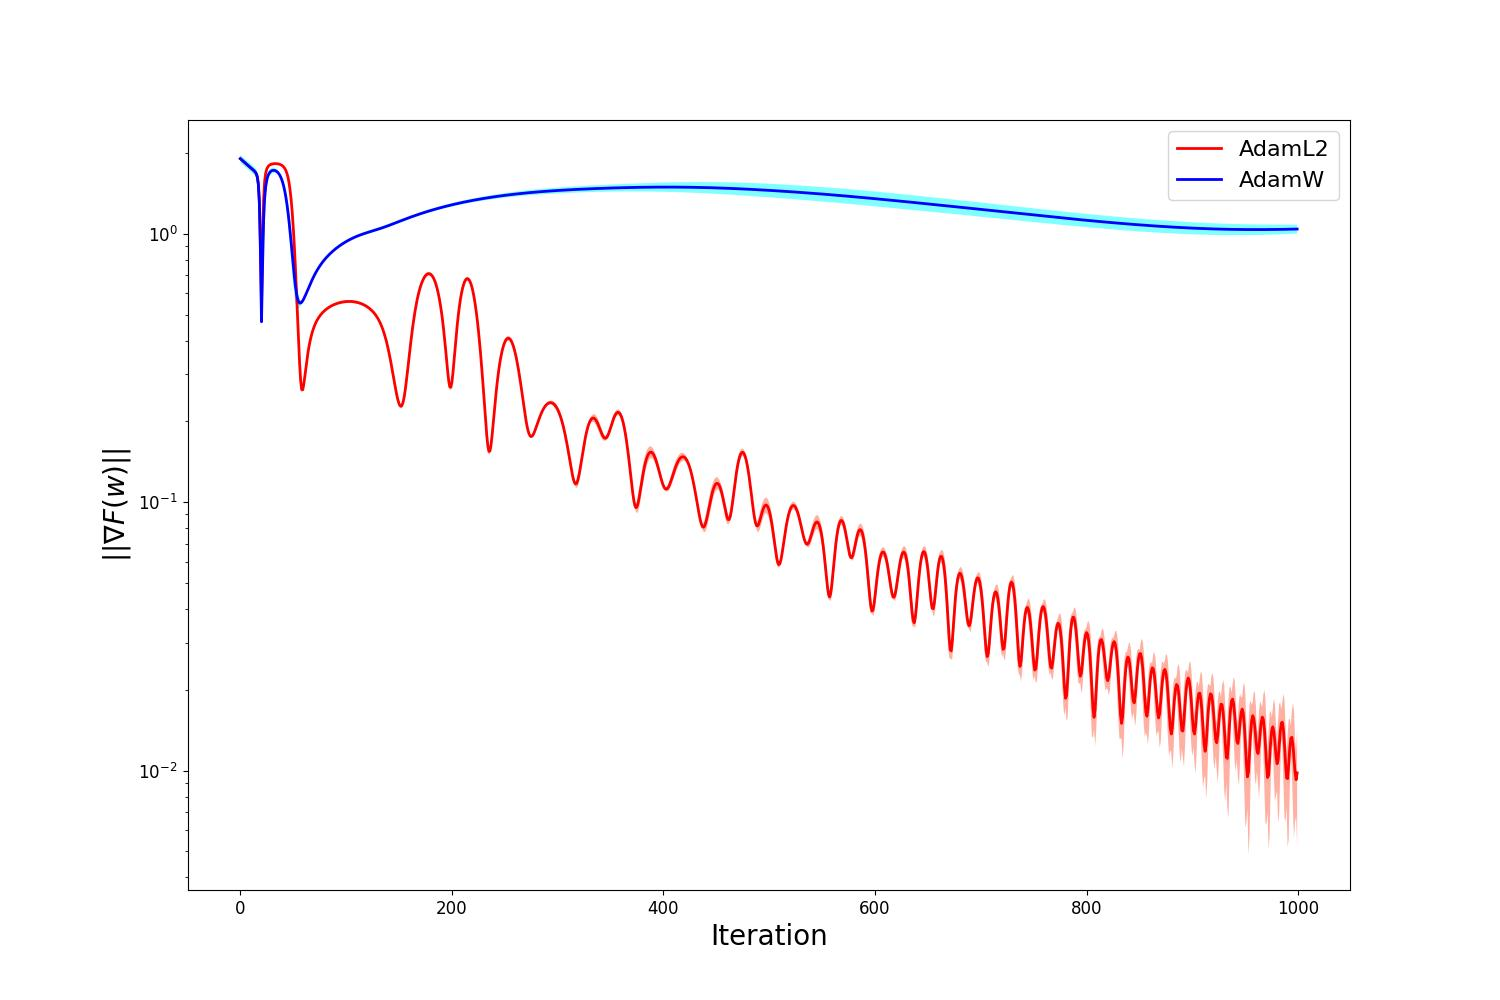
\includegraphics[width=0.7\linewidth]{pictures/fig1.jpg}
\captionsetup{justification=centering,margin=0.5cm}
\caption{Adam и AdamW по классическому критерию}
\label{fig:adams_errors}
\end{figure}

\begin{figure}[h!]
\centering
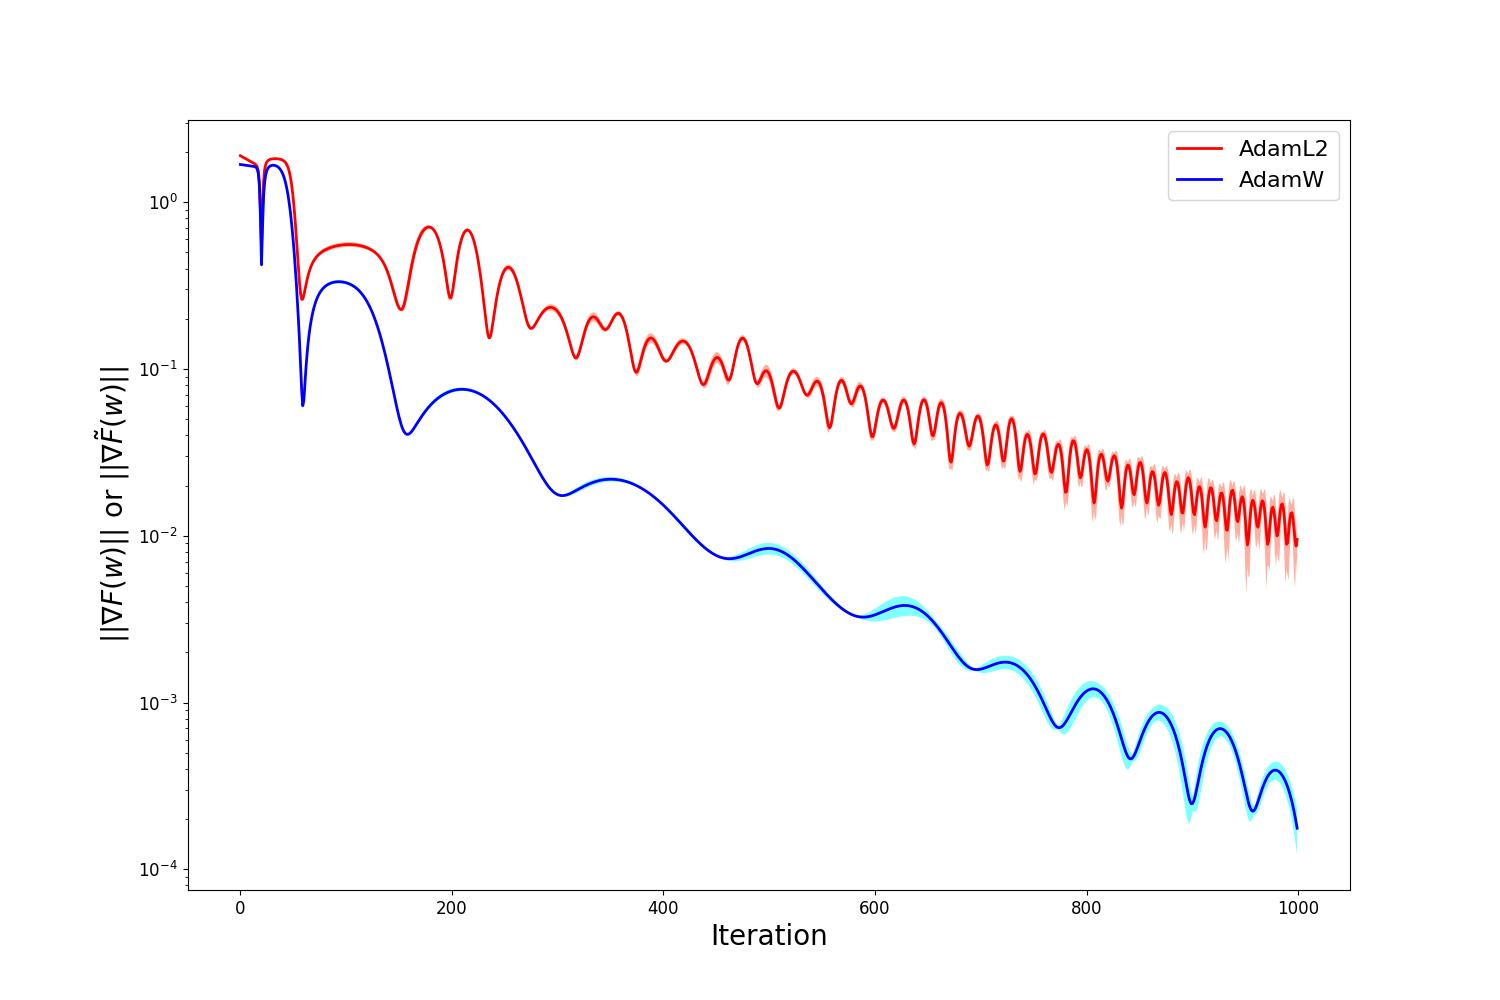
\includegraphics[width=0.7\linewidth]{pictures/fig2.jpg}
\captionsetup{justification=centering,margin=0.5cm}
\caption{Adam и AdamW с модифицированным критерием}
\label{fig:adams_special_errors}
\end{figure}

\begin{figure}[h!]
\centering
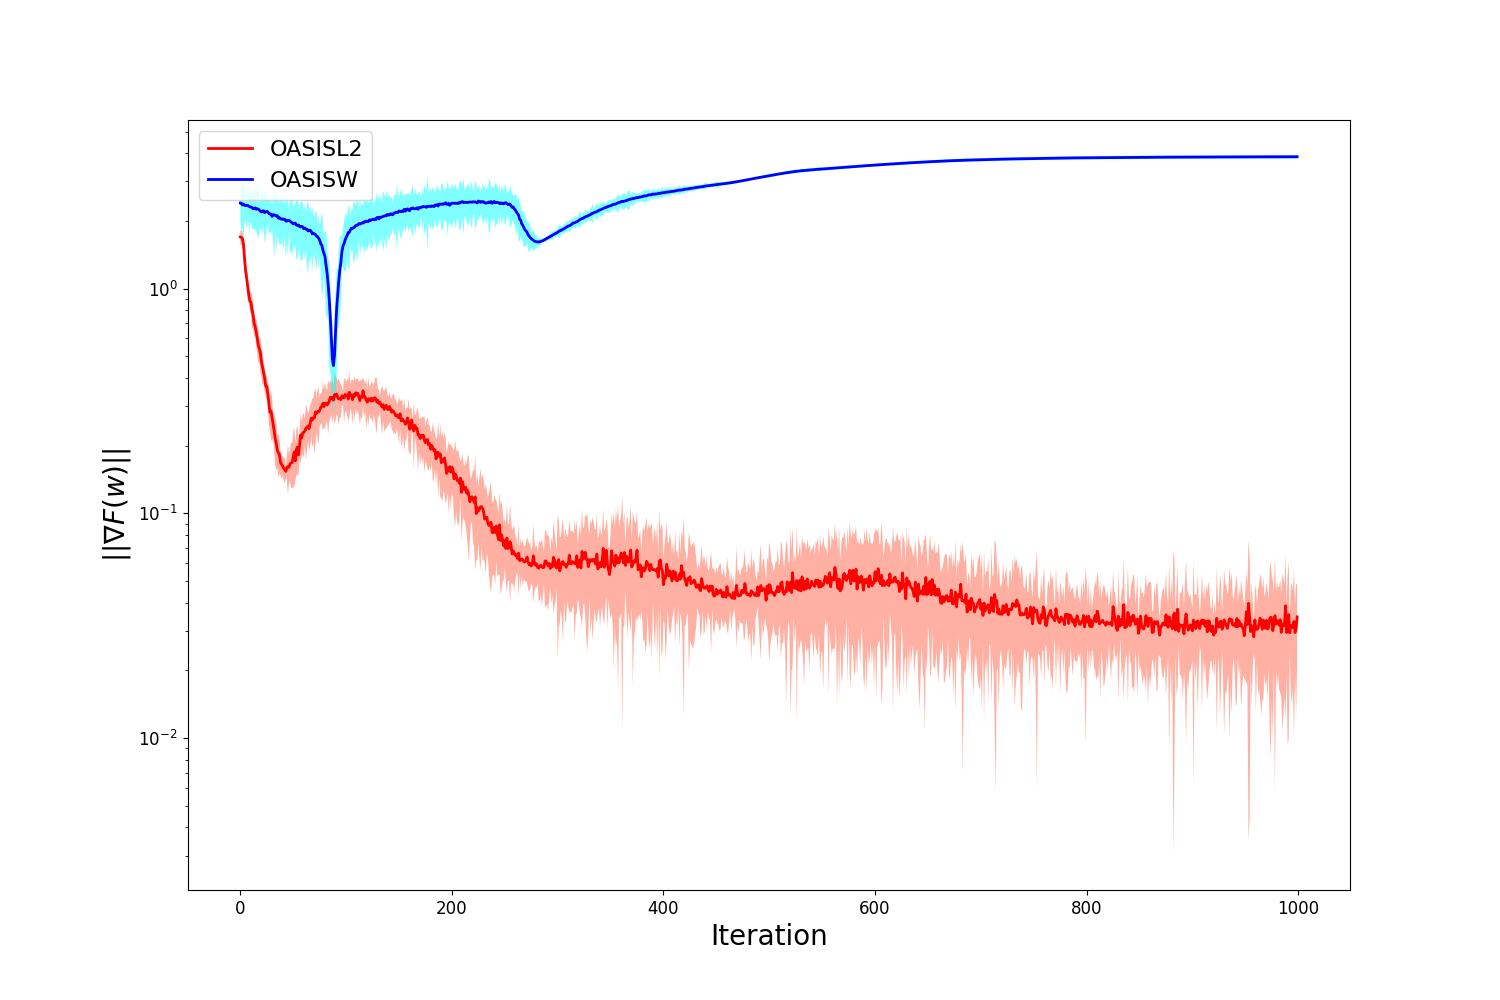
\includegraphics[width=0.7\linewidth]{pictures/fig1_oasis.jpg}
\captionsetup{justification=centering,margin=0.5cm}
\caption{OASIS и OASISW по классическому критерию}
\label{fig:oasis_errors}
\end{figure}

\begin{figure}[h!]
\centering
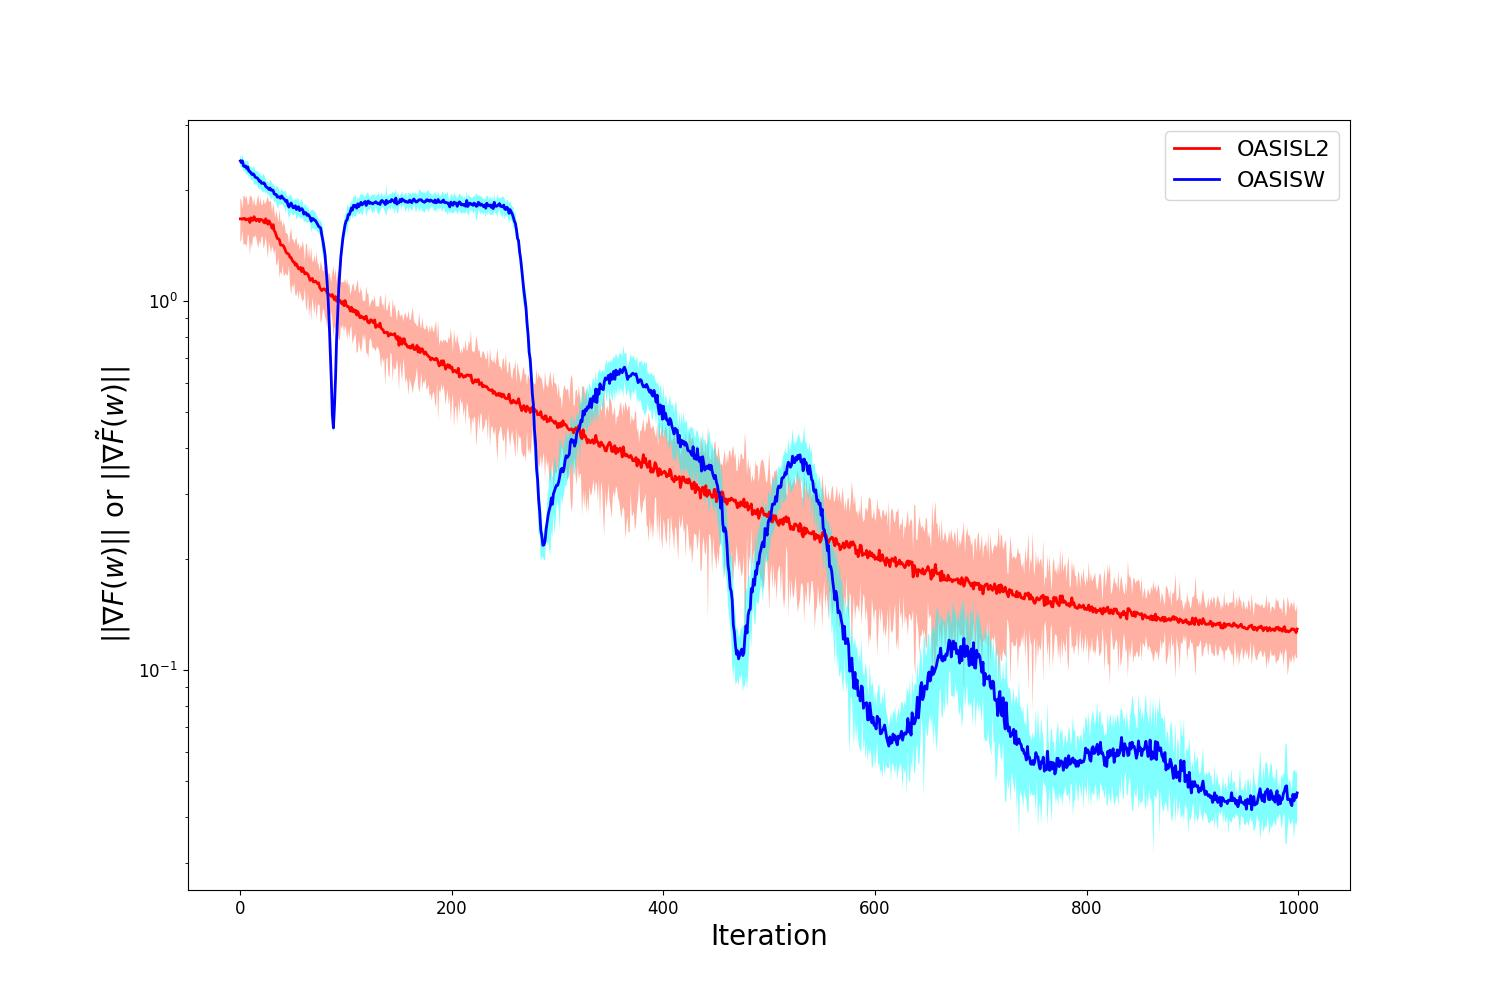
\includegraphics[width=0.7\linewidth]{pictures/fig2_oasis.jpg}
\captionsetup{justification=centering,margin=0.5cm}
\caption{OASIS и OASISW с модифицированным критерием}
\label{fig:oasis_special_errors}
\end{figure}

Нужно пояснить данные графики, в первой теореме мы приводим оценку сходимости необходимого количества шагов для нормы градиента измененной функции $\tilde{F}$. На графиках \ref{fig:adams_errors} и \ref{fig:oasis_errors} приведена норма градиента изначальной функции потерь от итерации, как видно из графиков норма изначального градиента для метода с затуханием весов не убывает с итерациями, на графиках \ref{fig:adams_special_errors} и \ref{fig:oasis_special_errors} построены графики для нормы градиента модифицированной функции потерь $\tilde{F}$. Различие сходимости в методах Adam и OASIS иллюстрирует выбранный критерий сходимости в первой теореме, это подтверждает, что методы с предобуславливанием и затуханием весов оптимизируют не функцию потерь $F$, а $\tilde{F}$. Именно градиент $\tilde{F}$ убывает с итерациями в то время, как градиент $F$ остается неизменным.

\begin{figure}[h!]
\centering
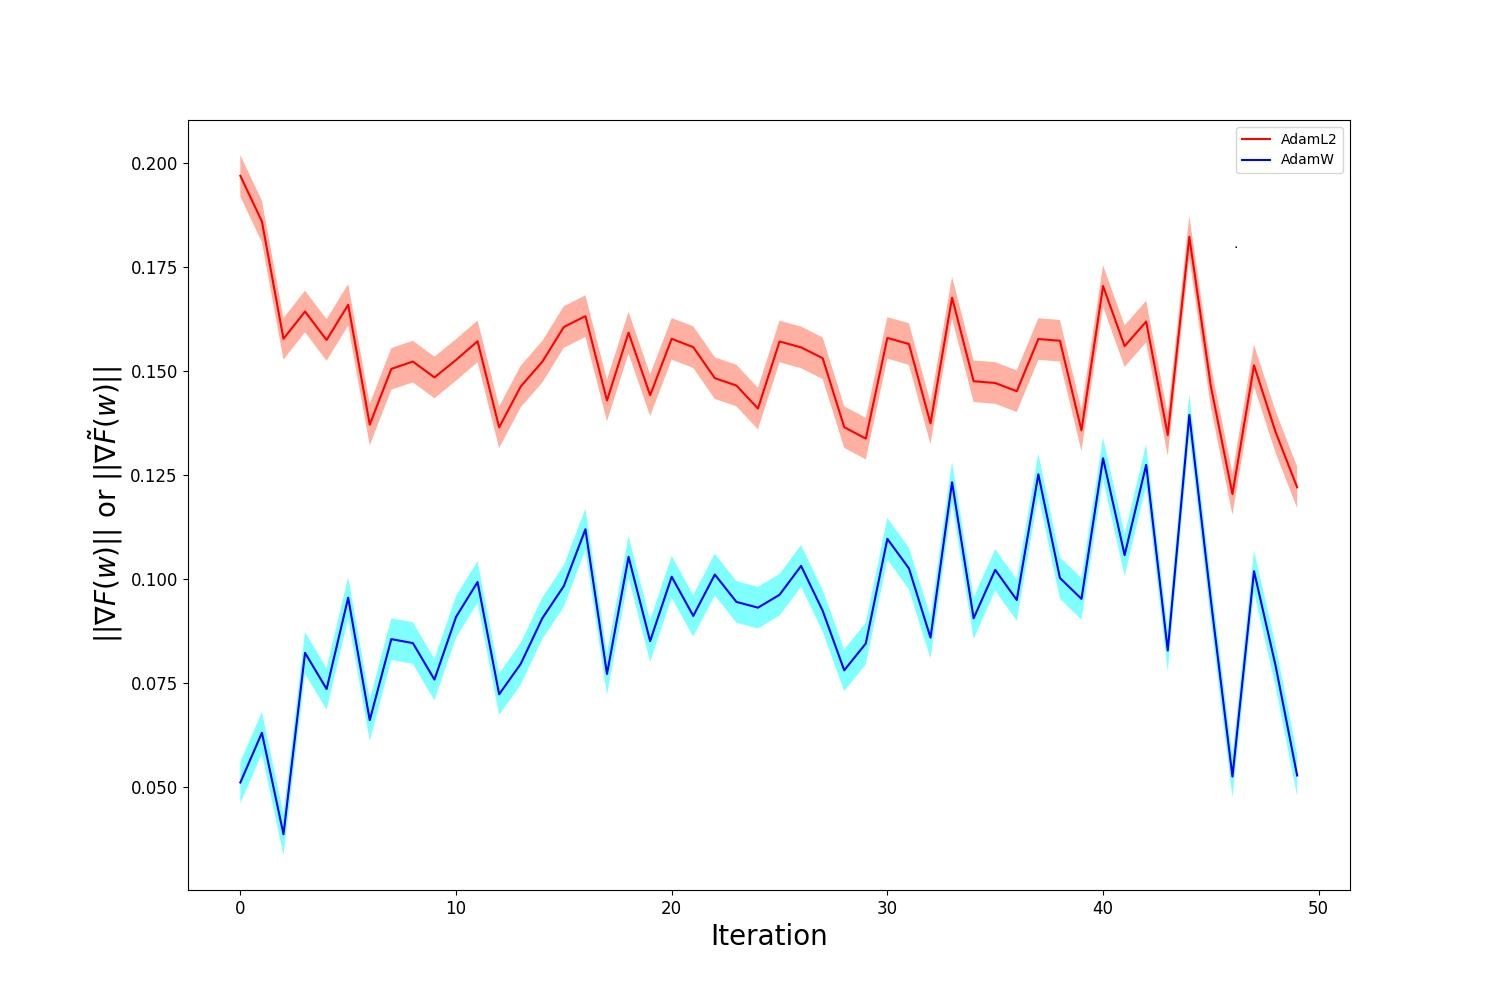
\includegraphics[width=0.7\linewidth]{pictures/net_ADAML2.jpg}
\captionsetup{justification=centering,margin=0.5cm}
\caption{Adam и AdamW по классическому критерию в слое нейронной сети}
\label{fig:adam_net_errors}
\end{figure}

\begin{figure}[h!]
\centering
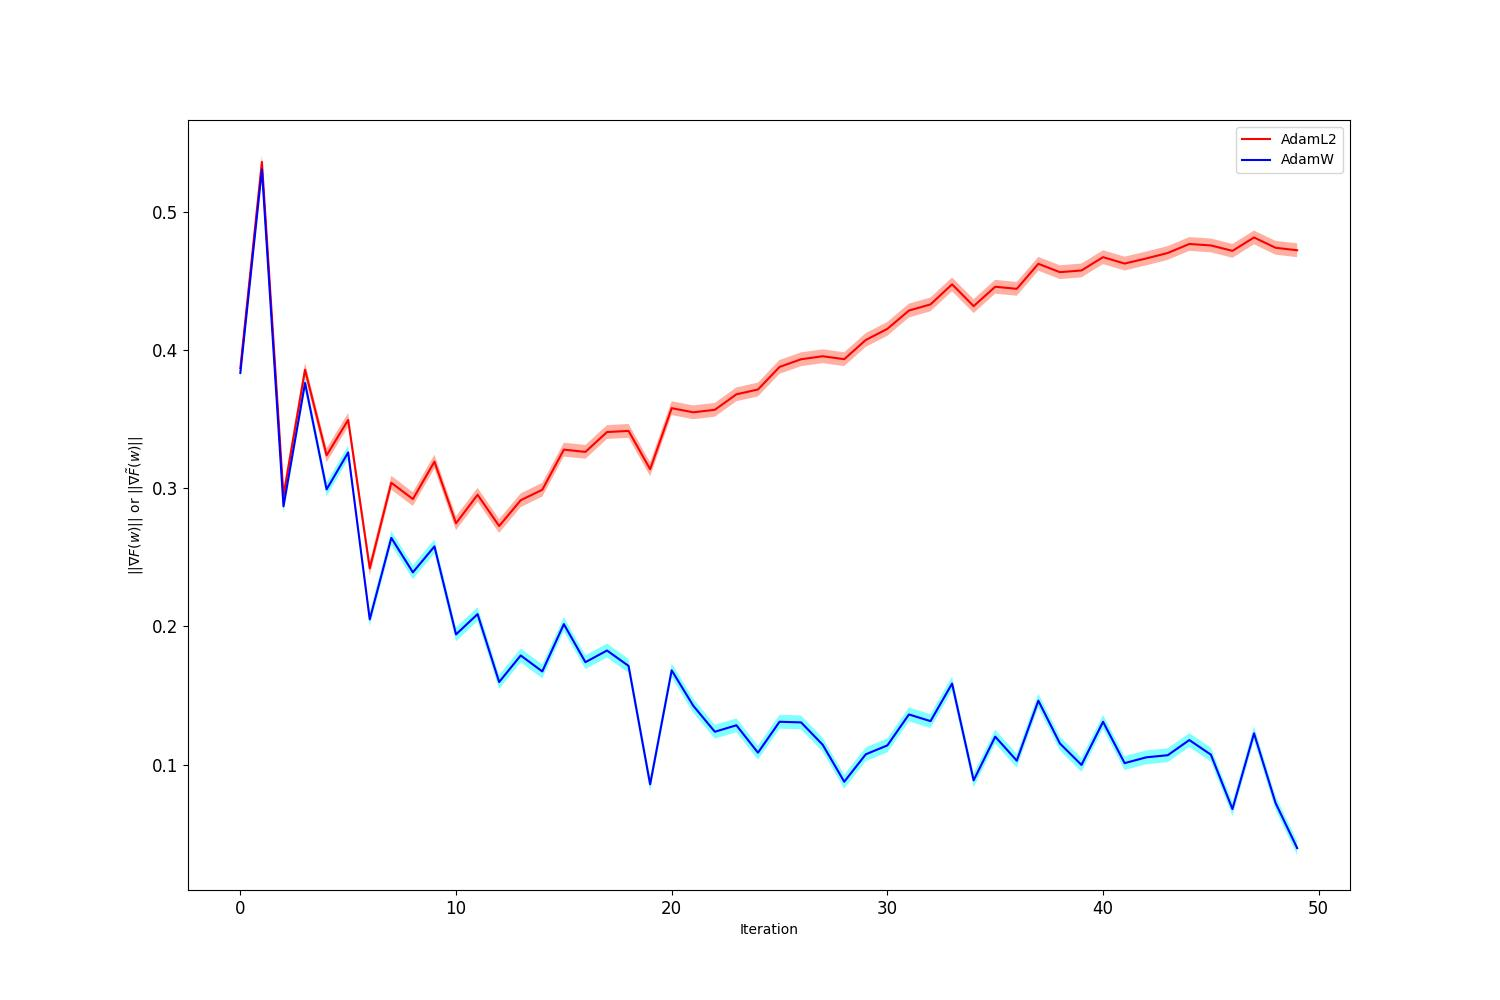
\includegraphics[width=0.7\linewidth]{pictures/net_ADAMW.jpg}
\captionsetup{justification=centering,margin=0.5cm}
\caption{Adam и AdamW с модифицированным критерием в слое нейронной сети}
\label{fig:adam_net_special_errors}
\end{figure}

Это явление можно наблюдать при обучении нейроных сетей на задачу классификации, в силу сложности современных нейронных сетей этот эффект наблюдается в отдельных слоях нейронной сети, но все таки он есть и он влияет на сходимость.